\subsection{Sejarah Perusahaan}

\begin{figure}[htbp]
    \centering
    % Logo Hexagon
    
\includegraphics[width=0.6\textwidth]{figures/logohexagon.png}
    \caption{PT Hexagon Karyatama Indonesia}
    \label{fig:PT Hexagon Karyatama Indonesia}
\end{figure}
PT Hexagon Karyatama Indonesia, yang dikenal secara komersial sebagai Hexagon Inc., didirikan dengan fokus pada penyediaan solusi digital kreatif dan teknologi informasi (IT solutions) di Indonesia. Perusahaan ini beroperasi di bidang digital artwork, pembuatan website, IT consultation, branding, digital marketing, dan media consulting, yang membantu berbagai klien bisnis memanfaatkan teknologi digital untuk meningkatkan visibilitas dan efektivitas usaha mereka. Hexagon Inc. awalnya berdiri sebagai entitas yang fokus pada layanan digital kreatif, lalu berkembang untuk mencakup konsultasi teknologi dan solusi IT yang lebih luas bagi sektor usaha kecil hingga menengah di Indonesia.

Perusahaan berlokasi di Cimahi, Jawa Barat, Indonesia, dengan tim yang relatif kecil namun berfokus pada inovasi desain dan teknologi untuk klien lokal. Nama Hexagon diambil sebagai bagian dari identitas merek, meskipun tidak berafiliasi langsung dengan Hexagon global yang bergerak di teknologi sensor/metrologi industri.


\subsection{Deskripsi Produk/Jasa}

Tata kelola perusahaan dalam Bahasa Inggris Corporate Governance, merujuk nilai-nilai inti (work values) yang menjadi kebijakan bagi pegawai dan budaya kerja perusahaan. Think Good menekankan pentingnya berpikir positif, menghasilkan ide-ide cemerlang, dan memberikan solusi yang efektif. Do Better menggambarkan komitmen untuk terus belajar, mengembangkan diri, melakukan perbaikan, serta menjadi versi terbaik dari individu maupun tim. Give the Best mendorong dedikasi penuh untuk memberikan hasil terbaik di setiap aspek pekerjaan dan memastikan setiap tindakan memberikan dampak positif. Adapun proses penerapan tata kelola perusahaan di PT. Hexagon Inc. seperti di bawah ini:

\begin{figure}[htbp]
    \centering
    % Work Values
    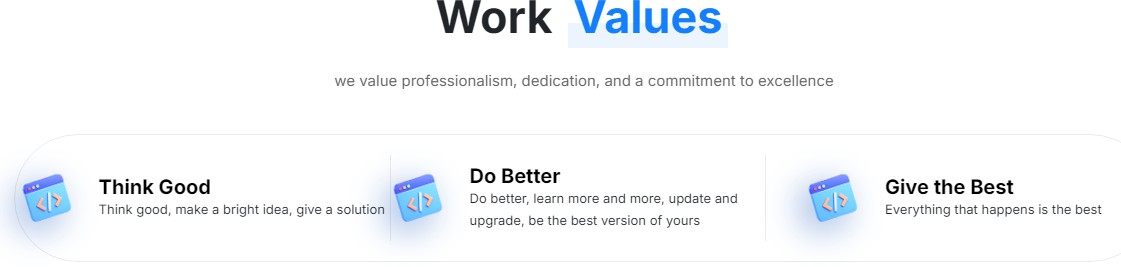
\includegraphics[width=0.6\textwidth]{figures/work_values_hexagon.png}
    \caption{Penerapan Tata Kelola Perusahaan}
    \label{fig:Penerapan Tata Kelola Perusahaan}
\end{figure}


\subsubsection{Strategi Perusahaan}

Strategi utama Hexagon Inc. berfokus pada beberapa hal berikut:

1. Pendekatan Customer-First

Perusahaan mengutamakan kepuasan klien melalui pendekatan yang berorientasi pada kebutuhan pelanggan, dengan berupaya memahami tujuan bisnis klien dan memberikan solusi digital yang sesuai.

2. Solusi Digital Terpadu

Hexagon Inc. menawarkan layanan yang terintegrasi, mulai dari konsultasi IT, desain web responsif, strategi digital marketing, hingga branding dan media consulting. Hal ini memungkinkan klien mendapatkan layanan lengkap dari satu penyedia solusi.

3. Kreativitas dan Strategi

Strategi perusahaan menekankan kombinasi kreativitas desain dengan strategi digital yang terukur untuk meningkatkan keterlibatan dan visibilitas brand klien di platform digital.

4. Teknologi Berbasis Trend Terkini

Dengan memanfaatkan platform teknologi modern dan tren digital seperti optimasi SEO, social media ads, serta pengembangan website yang responsif, Hexagon Inc. menerapkan strategi agar klien dapat bersaing di pasar digital yang cepat berubah.


\subsubsection{Visi dan Misi Perusahaan}

\textbf{Visi}

To be the leading provider of digital artwork and IT solutions, driving innovation and consistently exceeding client expectations.

(Tujuan untuk menjadi penyedia terkemuka solusi IT dan digital artwork yang mendorong inovasi serta secara konsisten melampaui ekspektasi klien.)

\textbf{Misi}

To grow businesses with integrity, delivering high-quality services that benefit both companies and their customers.

(Mengembangkan bisnis dengan integritas, memberikan layanan berkualitas tinggi yang memberikan manfaat bagi perusahaan dan pelanggan mereka.)


\subsection{Deskripsi Produk Jasa}

Hexagon telah membuat dan mengembangkan website dan aplikasi yang memenuhi standar industri, yang dibuat dan disusun oleh tim utama perusahaan Hexagon dengan ketelitian dan kerja sama demi menciptakan aplikasi dan website sesuai keinginan klien. Beberapa produk yang telah dikembangkan antara lain sistem aplikasi keuangan sekolah dan pesantren (Edutama) yang merupakan kerja sama dengan tiga sekolah yaitu SMK Negeri 1 Cianjur, SMK Negeri 2 Sumedang, dan SMK Negeri 46 Jakarta di bawah koordinasi BBPPMPV Bidang Mesin dan Teknik Industri, Kemendikbud RI. Selain itu terdapat aplikasi Jatidiri.app, yaitu sebuah superaplikasi psikologi yang bertujuan untuk membantu individu memahami diri mereka lebih baik. Dengan menggabungkan berbagai tes dan layanan, aplikasi ini memberikan wawasan tentang kepribadian, kecerdasan, dan potensi seseorang yang mudah diakses, terjangkau, dan dapat diandalkan. Kemudian terdapat aplikasi Berseka, yaitu aplikasi pengelolaan sampah yang memungkinkan pengguna menukarkan sampah menjadi poin yang dapat ditukarkan dengan berbagai macam produk.


\subsection{Struktur Organisasi}

\begin{figure}[htbp]
    \centering
    % Struktur Organisasi
    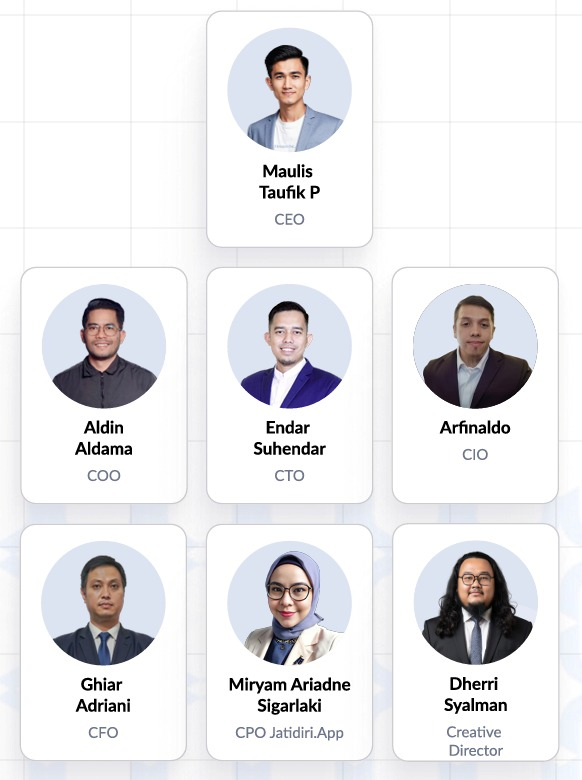
\includegraphics[width=0.6\textwidth]{figures/struktur_hexagon_1.png}
    \label{fig:Struktur Organisasi}
\end{figure}
\begin{figure}[htbp]
    \centering
    % Struktur Organisasi2
    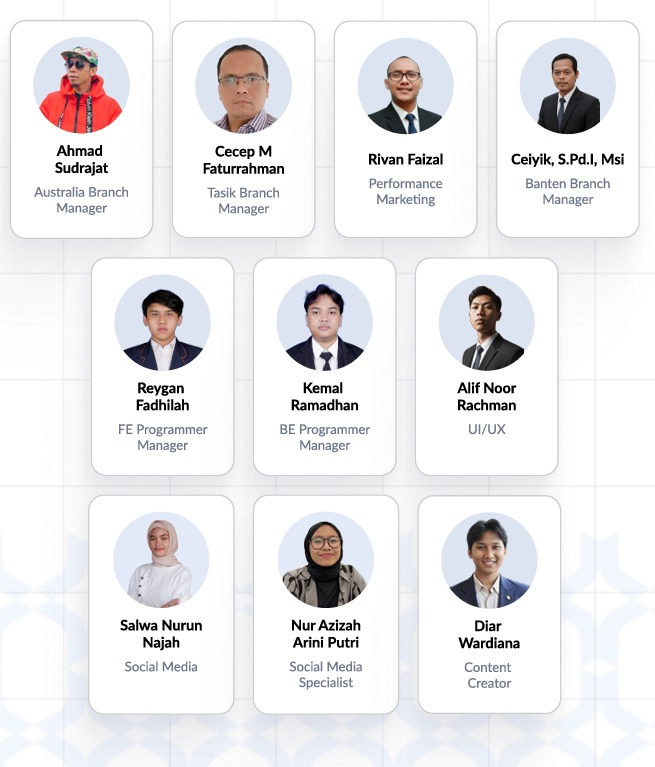
\includegraphics[width=0.6\textwidth]{figures/struktur_hexagon_2.png}
    \caption{Struktur Organisasi}
    \label{fig:Struktur Organisasi 2}
\end{figure}

CEO (Chief Executive Officer) bertugas memimpin organisasi secara keseluruhan, menentukan visi, strategi, dan mengambil keputusan strategis untuk keberlangsungan perusahaan. CTO (Chief Technology Officer) mengelola strategi teknologi perusahaan, memastikan pengembangan serta integrasi teknologi untuk mendukung bisnis. CMO (Chief Marketing Officer) bertanggung jawab atas pemasaran, branding, dan strategi komunikasi untuk meningkatkan awareness dan pencapaian penjualan. CFO (Chief Financial Officer) mengelola aspek keuangan perusahaan, termasuk anggaran, pelaporan keuangan, dan pengendalian operasional keuangan.

FE Programmer Manager bertugas memimpin pengembangan front-end aplikasi untuk memastikan antarmuka pengguna yang berkualitas. BE Programmer Manager mengawasi pengembangan back-end aplikasi guna memastikan sistem berjalan dengan optimal dan mendukung operasional bisnis. Branch Manager (Auxy) dan Branch Manager (Tasik) masing-masing bertanggung jawab mengelola kegiatan operasional cabang perusahaan di wilayah tertentu atau pada fokus tugas tertentu, sedangkan Head of SBU (Strategic Business Unit) memimpin unit bisnis strategis untuk mencapai target yang telah ditetapkan.

UI/UX Designer Manager bertugas mengawasi desain antarmuka dan pengalaman pengguna untuk memastikan produk yang mudah digunakan dan menarik secara visual. Creative Production dan Creative Director bekerja sama dalam merancang dan mengelola ide kreatif untuk kebutuhan konten visual dan strategi pemasaran, di mana Creative Director memimpin pengembangan konsep kreatif secara keseluruhan. Social Media Staff mengelola media sosial perusahaan dengan menciptakan konten yang menarik dan relevan untuk meningkatkan interaksi pengguna. Manager Digital Advertising bertanggung jawab atas perencanaan dan pelaksanaan kampanye iklan digital untuk meningkatkan visibilitas dan engagement online. Terakhir, Content Creation Staff berperan dalam menciptakan dan mengelola konten kreatif untuk mendukung komunikasi perusahaan di berbagai platform.
